\documentclass[9pt,twocolumn,twoside]{osajnl}
%% Please use 11pt if submitting to AOP
% \documentclass[11pt,twocolumn,twoside]{osajnl}
\usepackage{graphicx}
\usepackage{array}
\usepackage{amssymb}
\usepackage{lineno}
\usepackage{amsmath}
\usepackage{tabularx}
\usepackage{multirow}
\usepackage{rotating}
\usepackage{makecell}
\usepackage{xcolor}

\journal{josab} % Choose journal (ao, aop, josaa, josab, ol, pr)

% See template introduction for guidance on setting shortarticle option
\setboolean{shortarticle}{false}
% true = letter / tutorial
% false = research / review article
% (depending on journal).

\title{Talbot wavefront sensor measurement errors for partially coherent illumination}

\author[a, $\dagger$]{Andrii Goloborodko}
\affil[a]{Independent Researcher, 70-351, Szczecin, Poland}
\affil[$\dagger$]{a.a.goloborodko@gmail.com}
\author[b, $\ddagger$]{Myhailo Kotov}
\affil[b]{Taras Shevchenko National University of Kyiv, 64/13 Volodymyrska str., Kyiv, Ukraine}
\affil[$\ddagger$]{kotov.m@knu.ua}

%% To be edited by editor
% \dates{Compiled \today}

%\ociscodes{(140.3490) Lasers, distributed feedback; (060.2420) Fibers, polarization-maintaining;(060.3735) Fiber Bragg gratings.}

%% To be edited by editor
% \doi{\url{http://dx.doi.org/10.1364/XX.XX.XXXXXX}}

\begin{abstract}
\end{abstract}

\setboolean{displaycopyright}{true}

\begin{document}

\maketitle

\section{Introduction}
\label{sec:intro}

The Talbot self-imaging effect and the fractional Talbot phenomenon under continuous-wave illumination have many applications, including array illumination \cite{Zhou:01}, Lau cavities and phase locking of laser arrays \cite{Wang:16}, holographic multiplexed storage \cite{Zhao:01}, and many others \cite{Yuanhua_2014,Chavel:84, BOURIMBORDE1993397, 10.1117/1.1827608,Grizolli2017, Marathe2017,Yeganeh:13,McMorran_2009, Calogero19, PhysRevA.51.R14,NAKANO1990195, PhysRevLett.104.183901, Wang2010, Torcal-Milla2010, Zhang2015}. However, is the Talbot effect under incoherent illumination the same as that under continuous-wave illumination? To our knowledge, several papers have addressed this important question \cite{Liu:88, Teng:03}, but there is no information about the intermediate effects associated with the gradual disappearance of the Talbot phenomenon. For instance, Ref.~[\citenum{DUSEK1994203}] provides a preliminary analysis of the effects of spatial coherence on possible spectral changes in the far field. However, that study presents no closed-form expressions or numerical results, and Fresnel diffraction is not considered at all. In Ref.~[\citenum{Hoenders:05}], the van Cittert--Zernike theorem is generalized for weakly periodic media, and a numerical study of near-field changes in spatial coherence induced by a metal grating is presented in Ref.~[\citenum{Saastamoinen:13}]. Meanwhile, Ref.~[\citenum{Schouten:25}] predicts the generation of ``coherence carpets'' in the Fresnel zone.

 
The paper is organized as follows. \textcolor{red}{Section \ref{sec:diffraction} presents brief description of the Talbot image formation and the effect of bandwidth on the diffraction phenomenon. Section \ref{sec:result} presents numerical simulations and discussion. An analysis of the applicability of the model in case of phase gratings is provided in Section \ref{sec:limit}.} Finally, concluding remarks are given in Section \ref{sec:conclusion}.


\section{Talbot effect for finite-bandwidth illumination}
\label{sec:diffraction}
The Talbot, or self-imaging, effect is a near-field diffraction phenomenon in which a periodic structure illuminated by coherent light reproduces its spatial pattern at specific intervals, known as Talbot distances (see Fig.~\ref{fig.1}).
\begin{figure}[!ht]
\centering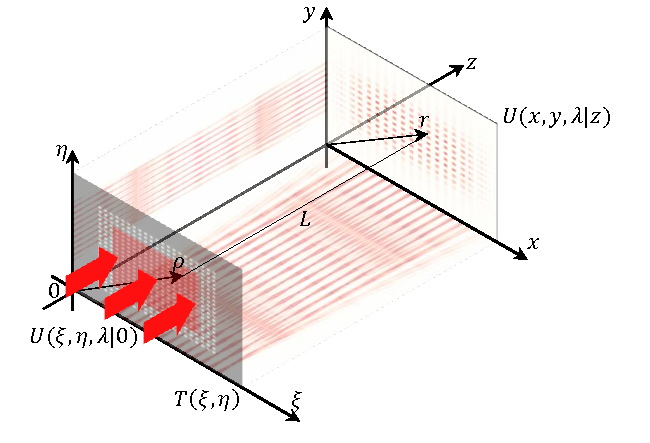
\includegraphics[width=8cm]{fig01_role.pdf}
\caption{Schematic diagram of light diffraction by a grating \cite{GOLOBORODKO20164478}. The grating is placed in the plane defined by coordinate $z=0$, and the CCD is situated in the plane defined by coordinate $Z$.}
\label{fig.1}
\end{figure}
Here and in what follows, the following conventions are adopted: $(\xi, \eta)$ represent the in-plane coordinates of the grating $G$, positioned in the plane $(\xi, \eta| 0)$; $(x, y)$ are the coordinates in the plane of the two-dimensional (2D) CCD, placed at a distance $Z$ from the grating. To refer consistently to these coordinate systems in different planes, the notations $(\xi,\eta | z)$ and $(x, y | z)$ are used, where the symbol ``$|$'' separates the transverse $(\xi,\eta)$ or $(x, y)$ components from the longitudinal $(z)$ component in three-dimensional space (see Fig.~\ref{fig.1}). Based on the mentioned notations, and according to the Huygens-Fresnel principle, the field distribution at any distance $Z$ can be expressed as~\cite{GOLOBORODKO2024171973, sci_rep}:
\begin{eqnarray}
U(x, y| Z)&=& {\mathrm{e}^{j\frac{2\pi Z}{\lambda}}} \sum\limits_{n,m}C_{n,m} \mathrm{e}^{-j2\pi\left(\frac{x}{D_x} n+\frac{y}{D_y} m+\frac{Z\lambda}{2}\left(\frac{n^2}{D_x^2}+\frac{m^2}{D_y^2}\right)\right)} \nonumber \\
&&\times \iint\limits_{-\infty}^{+\infty}  S\left(f_x, f_y\right)\mathrm{e}^{-j 2\pi\left(\left(x+\frac{\lambda Z}{D_x}n\right) f_x+\left(y+\frac{\lambda Z}{D_y}m\right) f_y\right)}
\nonumber \\
&&\times \mathrm{e}^{-j\pi\lambda Z\left(f_x^2+f_y^2\right)}\mathrm{d}f_x\mathrm{d}f_y ,
\label{eq.8}
\end{eqnarray}
where $\{C_{n,m}\}$ are the Fourier coefficients associated with the grating unit cell \cite{Goloborodko21}, $D_x$ and $D_y$ are the spatial periods of the grating along the $x$ and $y$ axes, $\lambda$ stands for the beam wavelength, $f_x$ and $f_y$ are spatial frequencies associated with beam spatial profile, described by its spatial spectrum $S\left(f_x, f_y\right)$. 

It is now evident that only in the case of a $\delta$-like spatial spectrum of the beam: $S\left(f_x, f_y\right)=\delta\left(f_x\right) \delta\left(f_y\right)$, or, in other words, for an infinite beam with a plane wavefront, the grating will produce self-images along the $x$ and $y$ axes at distances where the argument of the $n^2$ and $m^2$ terms in (\ref{eq.8}) becomes a multiple of $2\pi$ \cite{Kovalenko13}:
\begin{eqnarray}
Z_{T_\chi} & =&2\frac{D^2_\chi}{\lambda},
\end{eqnarray}
where $\chi$ define coordinate $x$ or $y$. In the case of $D_x=D_y=D$, the grating is fully reproduced at the Talbot distances since $Z_{T_x}=Z_{T_y}=Z_T$. It can be seen that the images depend on the convolution of the grating and beam spectra and different illuminating sources produce different intensity distributions~\cite{Born01}: $
I(x, y| Z)=\left|U(x, y| Z)\right|^2$. Since \eqref{eq.8} describes the diffraction phenomenon under various illumination conditions in a unified formulation it is used to describe coherence parameters of diffracted illumination.

Partial coherence theory uses the coherence of light in the temporal domain to describe the space--time correlation functions of light \cite{Mandel1995, Li:25}. Therefore, the temporal diffractive intensity distribution at any distance from grating G is given by \cite{Schouten:25}:
\begin{eqnarray}
I\left(x,y,t| Z\right)&=&\iint\limits_{-\infty}^{+\infty}  s\left(\omega_1, \omega_2\right)U(x, y, \omega_1| Z) U^*(x, y, \omega_2| Z)  \nonumber\\&&\times \mathrm{e}^{-j\left(\omega_1 -\omega_2\right)t}\mathrm{d}\omega_1\mathrm{d}\omega_2,
\label{eq.15}
\end{eqnarray}
where $s\left(\omega_1, \omega_2\right)$ stands for the cross-spectral density. Note that, although $\omega$ does not explicitly appear in the notation of Eq.~(\ref{eq.8}), the amplitude $U(x, y| Z)$ is in fact wavelength dependent. Using $\omega = 2\pi c/\lambda$, where $c$ is the speed of light, it can then be expressed as a function of $\omega$:
$U(x, y| Z)\xrightarrow{}U(x, y, \omega| Z)$.

In practice, the intensity observed distribution on the image plane is not time instantaneous: measured intensity is the time-averaged one. In this sense, the time-averaged intensity is of great significance, and can be achieved by integration of the time diffractive intensity distribution over time \cite{Mandel1995}:
\begin{eqnarray}
I\left(x,y| Z\right)&=&\int\limits_{-\infty}^{+\infty}  I\left(\omega\right)I(x, y, \omega| Z) \mathrm{d}\omega,
\label{eq.16}
\end{eqnarray}
where the cross-spectral density has been taken as
$s\left(\omega_1, \omega_2\right)=I\left(\omega_1\right)\delta\left(\omega_1-\omega_2\right)$ \cite{Mandel1995}, where $I\left(\omega\right)$ stands for the the intensity spectrum of the source, and the intensity is expressed as:
\begin{eqnarray}
I(x, y, \omega| Z)=U(x, y, \omega| Z)U^*(x, y, \omega| Z).
\label{eq.17}
\end{eqnarray}
It can be seen that the time-averaged diffraction images depend only on the intensity spectrum among all source parameters. Therefore, different illuminating sources produce different time-averaged intensity distributions. A Gaussian spectral intensity distribution is considered for finite-bandwidth illumination \cite{Born01}:
\begin{eqnarray}
I(\omega) = s_0 \mathrm{e}^{-\frac{(\omega-\omega_0)^2}{\Delta\omega^2}},
\qquad \omega\geq 0,
\label{eq:gaussian_spectrum}
\end{eqnarray}
where $\omega_0$ represents central source frequency, $\Delta\omega$ is the spectral half-width at the $\mathrm{e}^{-1}$ level of the maximum and the normalization constant $s_0$ is chosen such that $\int_0^{+\infty}S(\omega)\mathrm{d}\omega=1$. As one can see, the Talbot distance depends on frequency, and each spectral component reproduces the grating at a slightly different longitudinal position $Z$. The relative displacement between these monochromatic Talbot patterns increases with propagation distance, producing a progressive loss of the longitudinal self-imaging structure after spectral averaging. Fig.~\ref{fig.0} shows examples of self-image degradation for different Talbot planes.
\begin{figure}[!ht]
\centering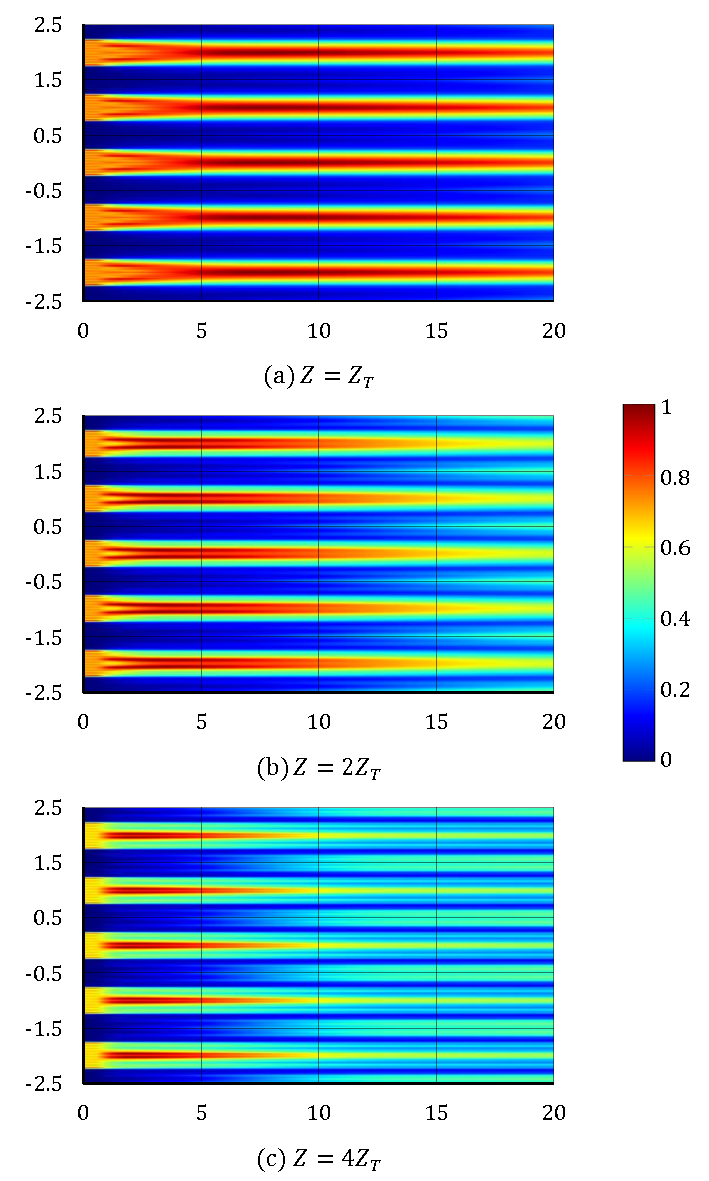
\includegraphics[width=8cm]{fig001.pdf}
\caption{2D map created on the basis of self-images cross sections the same $y = 0$ position at dependence on the source spectral half-widths $\Delta\omega$ for different Talbot lengths.}
\label{fig.0}
\end{figure}
It is visible, that if the spectral width of the source is relatively small $\Delta\omega/\omega_0<1\%$, the influence of the spectrum on the Talbot effect is slight. Additionally should be noted, that image sharpness, that can be seen in Fig.~\ref{fig.0}(a) for $\Delta\omega/\omega_0<2\%$, is also present in Figs.~\ref{fig.2}(b)-(c), but for smaller values of source spectral widths. Increasing of source spectral width, the spectral components are more abundant, and the effect of the spectrum on the Talbot phenomenon is greater because of dephasing of the different frequency components \cite{ao2027}. Further spectral width increasing will reveal needle-like structure connected with the grating period $D$, and constant image change with the distance, that characterize the self-imaging effect of the grating, will disappear. In addition, the distance from the grating to the observation plane also results in the variation of the diffraction intensity distribution of the grating at the same condition. So, if one want to observe self-imaging of the grating at the larger Talbot distances, the source with a smaller spectral width is mandatory.

\section{Simulation Results and Discussion}
\label{sec:result}

Capabilities of Talbot wavefront sensor are studied by simulating the corresponding experiment in accordance to the \eqref{eq.8} and \eqref{eq.16}. The simulated experimental setup is shown on Fig.~\ref{fig.2}. 
\begin{figure}[!ht]
\centering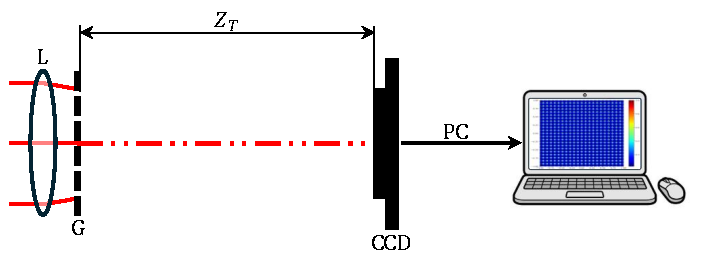
\includegraphics[width=8.5cm]{fig002.pdf}
\caption{Schematic diagram of the Talbot wavefront sensor used at the simulation.}
\label{fig.2}
\end{figure}
The diffraction grating (G) is illuminated by the light source with spectrum and arbitrary wavefront defined by lens (L). Talbot image is registered by a photodetector (CCD) located at the Talbot distance $Z_T$. The simulation consisted of the following consecutive stages: wavefront initialization, calculation of the image illuminance in the first Talbot plane, determination of local displacements of image points and wavefront reconstruction, comparison of the restored and input wavefronts. The measurement possibilities for spherical and astigmatic wavefronts were analyzed for sources having different spectra. 


\section{Model limitations}
\label{sec:limit}



\section{Conclusions}
\label{sec:conclusion}




\section*{Disclosures}
The authors declare no conflicts of interest.

\section*{Data availability}
The data underlying the results presented in this paper are not publicly available at this time but may be obtained from the authors upon reasonable request.

% Bibliography
\bibliography{sample}

% Full bibliography added automatically for Optics Letters submissions; the following line will simply be ignored if submitting to other journals.
% Note that this extra page will not count against page length
\bibliographyfullrefs{sample}

%Manual citation list
%\begin{thebibliography}{1}
%\bibitem{Zhang:14}
%Y.~Zhang, S.~Qiao, L.~Sun, Q.~W. Shi, W.~Huang, %L.~Li, and Z.~Yang,
% \enquote{Photoinduced active terahertz metamaterials with nanostructured
%vanadium dioxide film deposited by sol-gel method,} Opt. Express \textbf{22},
%11070--11078 (2014).
%\end{thebibliography}

% Please include bios and photos of all authors for aop articles
\ifthenelse{\equal{\journalref}{aop}}{%
\section*{Author Biographies}
\begingroup
\setlength\intextsep{0pt}
\begin{minipage}[t][6.3cm][t]{1.0\textwidth} % Adjust height [6.3cm] as required for separation of bio photos.
\begin{wrapfigure}{L}{0.25\textwidth}
\includegraphics[width=0.25\textwidth]{john_smith.eps}
\end{wrapfigure}
\noindent
{\bfseries John Smith} received his BSc (Mathematics) in 2000 from The University of Maryland. His research interests include lasers and optics.
\end{minipage}
\begin{minipage}{1.0\textwidth}
\begin{wrapfigure}{L}{0.25\textwidth}
\includegraphics[width=0.25\textwidth]{alice_smith.eps}
\end{wrapfigure}
\noindent
{\bfseries Alice Smith} also received her BSc (Mathematics) in 2000 from The University of Maryland. Her research interests also include lasers and optics.
\end{minipage}
\endgroup
}{}

\end{document}

